% Fault-phase availability analysis of Exp 3 and Exp 5 (Habib Hasanov, results analysis owner).
% Offered to Person 3 for \input in section 7.3 (or section 6). Every value comes from
% analysis/summarize.py: \expfault{..} in generated/exp46_numbers.tex, Table~\ref{tab:fault-phases}
% and Table~\ref{tab:detection} in generated/fault_tables.tex, and the figure from analysis/plots.py.
\providecommand{\expfault}[1]{\ifcsname expfault@#1\endcsname\csname expfault@#1\endcsname\else\textbf{[make figures]}\fi}
\InputIfFileExists{generated/exp46_numbers.tex}{}{}

\subsubsection*{Availability inside the fault window}
Whole-run success rates mix healthy and faulty periods. Splitting the availability-probe
operations of Exp 3 and Exp 5 at the injection and restart/heal commands in
\texttt{results/logs/chaos\_events.csv} isolates the fault window
(Table~\ref{tab:fault-phases}, Fig.~\ref{fig:fault-timeline}). With one node killed (3a), ONE
and QUORUM kept \expfault{3a-fault-ONE}\,\% and \expfault{3a-fault-QUORUM}\,\% success while ALL
dropped to \expfault{3a-fault-ALL}\,\%: first as timeouts until gossip declared the node down
(about \expfault{det-kill}\,s), then as immediate \texttt{Unavailable}. In 3b the second kill
followed the first by about 19\,s, so QUORUM succeeded until the second node failed and
\expfault{3b-fault-QUORUM}\,\% over the whole window, while ONE stayed at
\expfault{3b-fault-ONE}\,\%. ALL recovered only some seconds \emph{after} the restart command,
when the node had rejoined, so the ``after'' phase still contains failures.

\paragraph{Client-side unavailability under partition}
In Exp 5 the server-side behaviour matched the design (the majority accepted QUORUM writes),
but in each of the \expfault{exp5-stuck-runs} repetitions one probe level whose key had cass3
as first replica (\expfault{exp5-stuck-levels}) sent its requests to the isolated cass3 and
waited for the 5\,s client timeout, \expfault{exp5-stuck-timeouts} times in total, until the
partition healed. Every one of these requests was coordinated by cass3; a disconnected
container drops packets without resetting the client's TCP connections, which is the likely
reason the driver kept routing to it, and with retries disabled each such request failed. Pooled over repetitions
this is hidden (ONE \expfault{partition-fault-ONE}\,\%, QUORUM \expfault{partition-fault-QUORUM}\,\%),
but for the affected client the level was unavailable for over a minute although the cluster
could serve it. Availability in the CAP sense is therefore a property of the client's route as
well as of the replica set; a retry or speculative-execution policy that moves to the next
replica after a timeout would have masked it.

% Generated by analysis/summarize.py - do not edit by hand.
\begin{table}[t]\centering\footnotesize\setlength{\tabcolsep}{3pt}
\caption{Availability-probe success rate per consistency level and fault phase (Exp 3 and 5; repetitions pooled; ``fault'' = from the injection command to the restart/heal command).}\label{tab:fault-phases}
\begin{tabular}{llrrr}\hline
Run & Phase & ONE (\%) & QUORUM (\%) & ALL (\%) \\ \hline
exp3 3a & before & 100.0 & 100.0 & 100.0 \\
exp3 3a & fault & 100.0 & 100.0 & 4.7 \\
exp3 3a & after & 100.0 & 100.0 & 92.1 \\
exp3 3b & before & 100.0 & 100.0 & 100.0 \\
exp3 3b & fault & 99.9 & 60.1 & 2.0 \\
exp3 3b & after & 100.0 & 100.0 & 82.2 \\
exp3 3c & before & 100.0 & 100.0 & 100.0 \\
exp3 3c & fault & 100.0 & 100.0 & 5.3 \\
exp3 3c & between & 100.0 & 100.0 & 64.2 \\
exp3 3c & after & 100.0 & 100.0 & 93.9 \\
exp5 partition & before & 100.0 & 100.0 & 100.0 \\
exp5 partition & fault & 95.6 & 98.8 & 7.1 \\
exp5 partition & after & 98.9 & 99.5 & 98.3 \\
\hline\end{tabular}\end{table}

\begin{table}[t]\centering\footnotesize\setlength{\tabcolsep}{3pt}
\caption{Gossip failure-detection time (fault command to ``is now DOWN/UP'' in a peer's log).}\label{tab:detection}
\begin{tabular}{lrrrr}\hline
Fault (transition) & $n$ & mean (s) & min (s) & max (s) \\ \hline
kill (down) & 13 & 19.63 & 18.87 & 22.19 \\
partition, majority view & 4 & 19.19 & 18.75 & 19.38 \\
partition, minority view & 4 & 18.75 & 18.10 & 19.24 \\
start (up) & 16 & 9.85 & 7.25 & 11.12 \\
stop (down) & 3 & 0.67 & 0.54 & 0.81 \\
\hline\end{tabular}\end{table}



\begin{figure*}[t]\centering
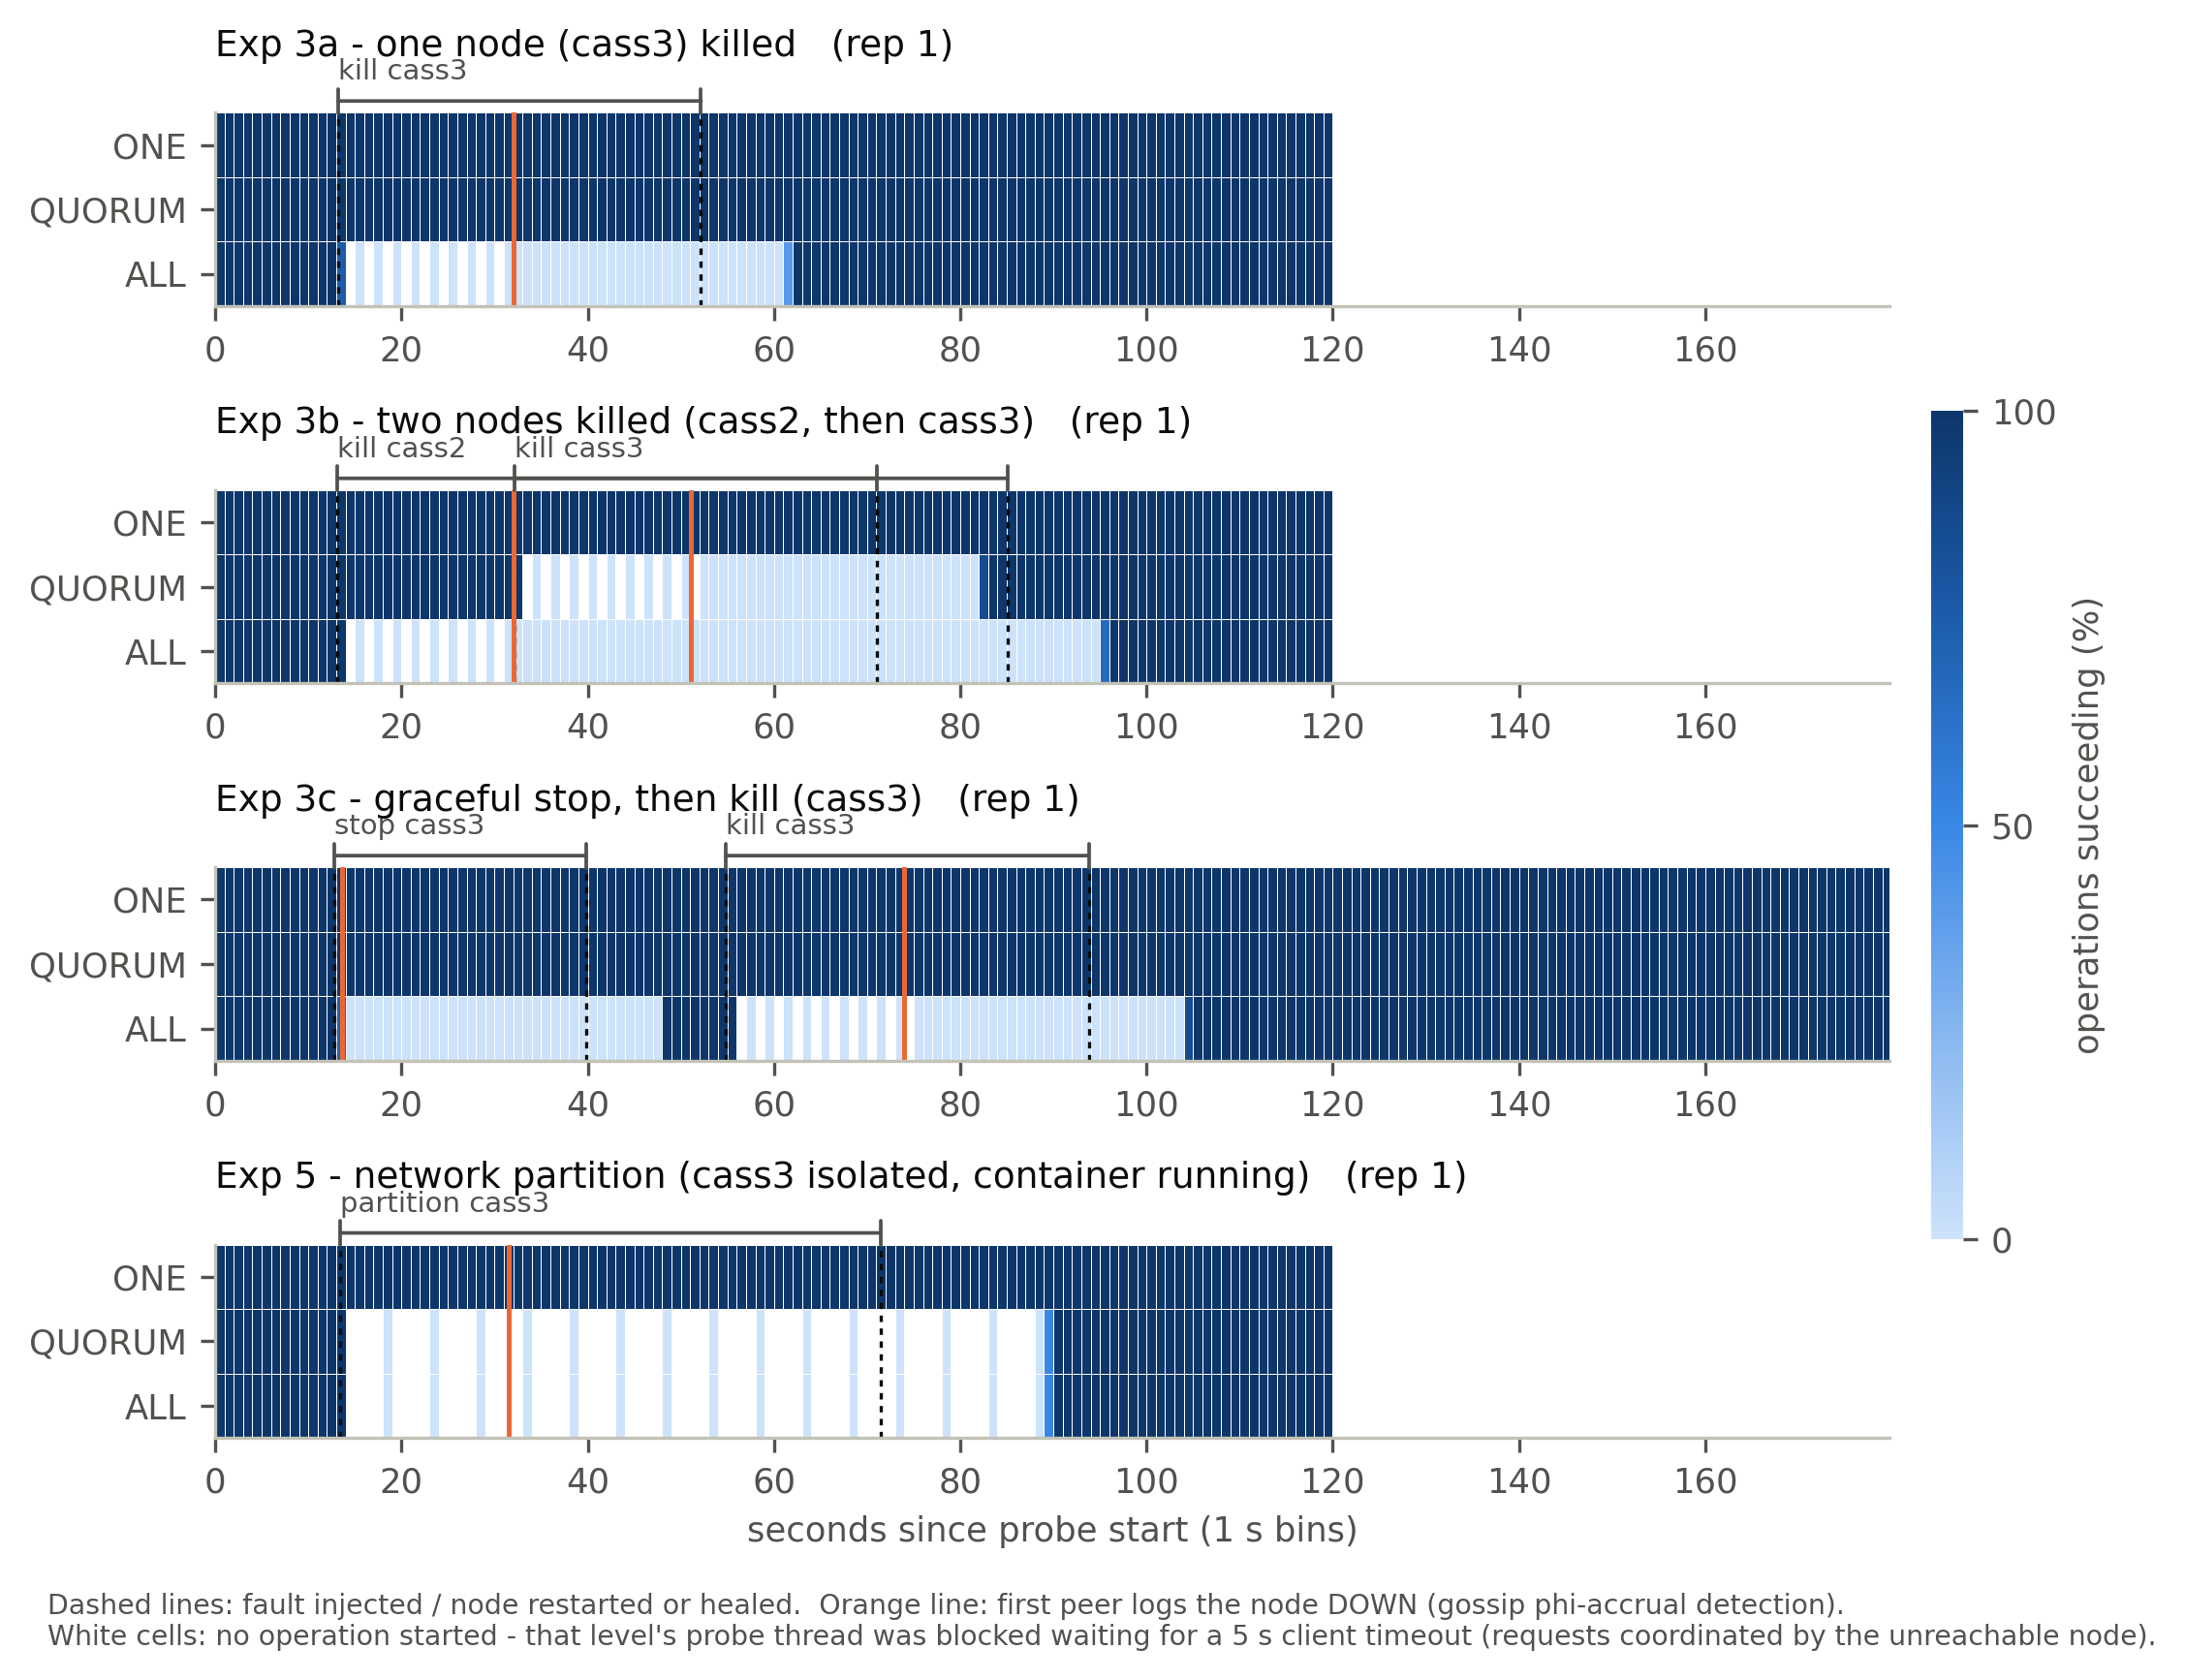
\includegraphics[width=\textwidth]{fault_availability_timeline.png}
\caption{Per-second success of the ONE/QUORUM/ALL availability probe in repetition 1 of each
fault scenario. Dashed lines: fault injected and node restarted/healed; orange: first peer
logs the node DOWN. White cells: the probe of that level was blocked on a 5\,s client
timeout.}\label{fig:fault-timeline}
\end{figure*}
